\documentclass[conference]{IEEEtran}
\IEEEoverridecommandlockouts

\usepackage[T1]{fontenc}
\usepackage[utf8]{inputenc}
\usepackage{cite}
\usepackage{amsmath,amssymb,amsfonts}
\usepackage{graphicx}
\usepackage{textcomp}
\usepackage{xcolor}
\usepackage{booktabs}
\usepackage{array}
\usepackage{multirow}
\usepackage{url}
\usepackage{float}
\usepackage{hyperref}
\usepackage{tikz}
\usetikzlibrary{shapes.geometric, arrows.meta, positioning, fit, backgrounds, calc}

\hypersetup{
    colorlinks=true,
    linkcolor=blue,
    citecolor=blue,
    urlcolor=blue
}

\begin{document}

\title{Regime-Specific Regression for NTL-Based Population Proxies: Urban-Rural Stratification Without Auxiliary Data}

\author{
\IEEEauthorblockN{Oishik Kar}
\IEEEauthorblockA{
\textit{Department of Computer Science and Engineering}\\
\textit{IIIT Dharwad, Karnataka, India}\\
23bcs089@iiitdwd.ac.in}
\and
\IEEEauthorblockN{Sunil C K}
\IEEEauthorblockA{
\textit{Assistant Professor}\\
\textit{Department of Computer Science and Engineering}\\
\textit{IIIT Dharwad, Karnataka, India}\\
sunil@iiitdwd.ac.in}
}

\maketitle

\begin{abstract}
Accurate sub-national population estimates are needed for resource allocation and tracking progress toward the Sustainable Development Goals, yet recent census data is unavailable in many countries. Night-time light (NTL) satellite imagery offers a low-cost alternative, but existing approaches fit a single regression across all administrative units, ignoring the structural difference between urban and rural settlement regimes. We propose a data-driven stratification method that uses KMeans clustering ($k{=}2$) on district-level NTL features to separate urban and rural units, then fits independent log-linear models for each group. The stratification label is derived entirely from freely available VIIRS data, requiring no census or land-cover inputs.

We validate the method on 670 Indian districts and 695 Nigerian Local Government Areas using VIIRS VNL V2.1 composites (2019) and WorldPop gridded population. In India, stratification raises cross-validated $R^2$ from 0.829 to 0.858 ($p{=}0.027$, paired $t$-test, 5 folds). In Nigeria, the absolute $R^2$ is lower (0.168 to 0.251, $p{=}0.004$), which we attribute to persistent gas flares in the Niger Delta, urban sensor saturation in Lagos, and low rural electrification in northern states; the method still produces the largest relative gain (+50\%), confirming that stratification matters most where structural heterogeneity is greatest.

Ablation experiments confirm that district area is not a confound ($r{=}0.119$), that area-normalised NTL density is counter-productive, and that adding NDVI as a covariate fails in tropical regions with dispersed settlement (e.g., Kerala). All code and data are publicly available, making the pipeline directly replicable for other countries with global VIIRS coverage.
\end{abstract}

\begin{IEEEkeywords}
night-time lights, VIIRS, population estimation, urban-rural stratification, KMeans, remote sensing
\end{IEEEkeywords}

%=============================================================================
\section{Introduction}
%=============================================================================

Accurate, timely population data is central to public policy: disaster response, vaccine distribution, electoral delimitation, infrastructure planning, and poverty targeting. Census data is expensive, slow, and in many low- and middle-income countries critically outdated. India's last full census was conducted in 2011; Nigeria's in 2006. The gap between official population counts and ground reality now spans over a decade in both countries.

Night-time light (NTL) satellite imagery is a practical alternative. Artificial lighting at night correlates strongly with human settlement density and economic activity~\cite{sutton1997}. The VIIRS Day/Night Band (DNB), operational since 2012, provides global coverage at approximately 500\,m resolution with monthly composites, making it one of the few freely available proxies for human presence at sub-national scale~\cite{elvidge2021}.

The standard approach in the literature is to sum or average radiance over administrative units, log-transform both NTL and population to handle their power-law distributions, and fit a single linear regression. This has produced reported $R^2$ values between 0.7 and 0.9 across various national studies. The single-model approach, however, assumes that the relationship between light and population is uniform across all district types. We show this assumption does not hold and that it causes systematic prediction errors in both dense urban cores and sparsely lit rural areas.

Urban and rural districts operate under different NTL regimes. In dense cities, the VIIRS sensor saturates (it reaches its dynamic range limit and records lower radiance than the true value), which causes it to underestimate urban population~\cite{elvidge2017}. Rural districts with dispersed agricultural populations may have near-zero NTL despite substantial population. A single regression fitted through both regimes is biased at both ends.

This paper makes three contributions. First, we propose using KMeans clustering on NTL features to generate urban/rural labels without any external classification data, then fitting separate regression models per cluster. Second, we validate the improvement using 5-fold cross-validation with paired $t$-tests rather than a single held-out $R^2$, which directly tests whether stratification consistently helps across data subsets. Third, we test on two structurally different countries (India and Nigeria) to check whether the improvement generalizes. We also run ablation experiments on area normalization, NDVI as an auxiliary feature, and district-size confounding.

%=============================================================================
\section{Related Work}
%=============================================================================

Early NTL-population research established the log-linear relationship using DMSP-OLS data~\cite{elvidge1997,lo2001}. The shift to VIIRS improved sensitivity at low radiances and reduced saturation in bright areas, though saturation remains a problem in the largest megacities~\cite{elvidge2021}. More recent work has incorporated auxiliary covariates such as road network density, land cover, and building footprint data~\cite{stevens2015}, but these studies typically fit a single model across all districts rather than stratifying.

Some papers have stratified by administrative tier or land cover class before modeling, but they depend on external classification inputs (official urban designations, land-cover maps) that may be unavailable, outdated, or inconsistently defined across countries. Our approach uses only the NTL raster, so it can be applied to any country with VIIRS coverage without additional data.

Area confounding in NTL-based models has been acknowledged but rarely tested directly. We test it explicitly with a correlation analysis. NDVI has been proposed as a corrective covariate for rural areas~\cite{zhang2013}, but its behaviour in tropical dispersed-settlement regions has not been studied. We find it is harmful in such contexts.

%=============================================================================
\section{Data}
%=============================================================================

\subsection{Night-Time Light Data}

We use the VIIRS VNL V2.1 Annual Composite for 2019, specifically the \texttt{average\_masked} variant obtained from the Earth Observation Group (EOG) at the Colorado School of Mines~\cite{elvidge2021}. This product is derived from monthly cloud-free composites filtered to remove ephemeral lights, background noise, and aurora contamination. The \texttt{average\_masked} variant additionally zeros out non-lit background pixels. Resolution is 15 arc-seconds (approximately 500\,m at the equator). Units are nW/cm$^2$/sr.

\subsection{Population Ground Truth}

Population data comes from WorldPop 2019 UN-adjusted 1\,km gridded estimates~\cite{worldpop2019}, downloaded separately for India and Nigeria. WorldPop integrates census microdata with satellite-derived covariates to produce consistent sub-national population grids. We use zonal statistics to aggregate pixel-level counts to Level~2 administrative boundaries.

\subsection{Administrative Boundaries}

District boundaries are taken from GADM v4.1 Level~2 shapefiles for both countries. India has 676 Level~2 units (districts); Nigeria has 775 (Local Government Areas). After removing units with zero NTL sum or zero estimated population, we retain 670 Indian districts and 695 Nigerian LGAs for analysis.

\subsection{Auxiliary Data}

MODIS MOD13A3 monthly NDVI composites for 2019 were obtained for India to test vegetation density as a corrective covariate. District-level mean NDVI was computed using zonal statistics after applying the standard scale factor of 0.0001.

% --- STUDY AREA MAP: two-column figure placed near top of page ---
\begin{figure*}[!t]
    \centering
    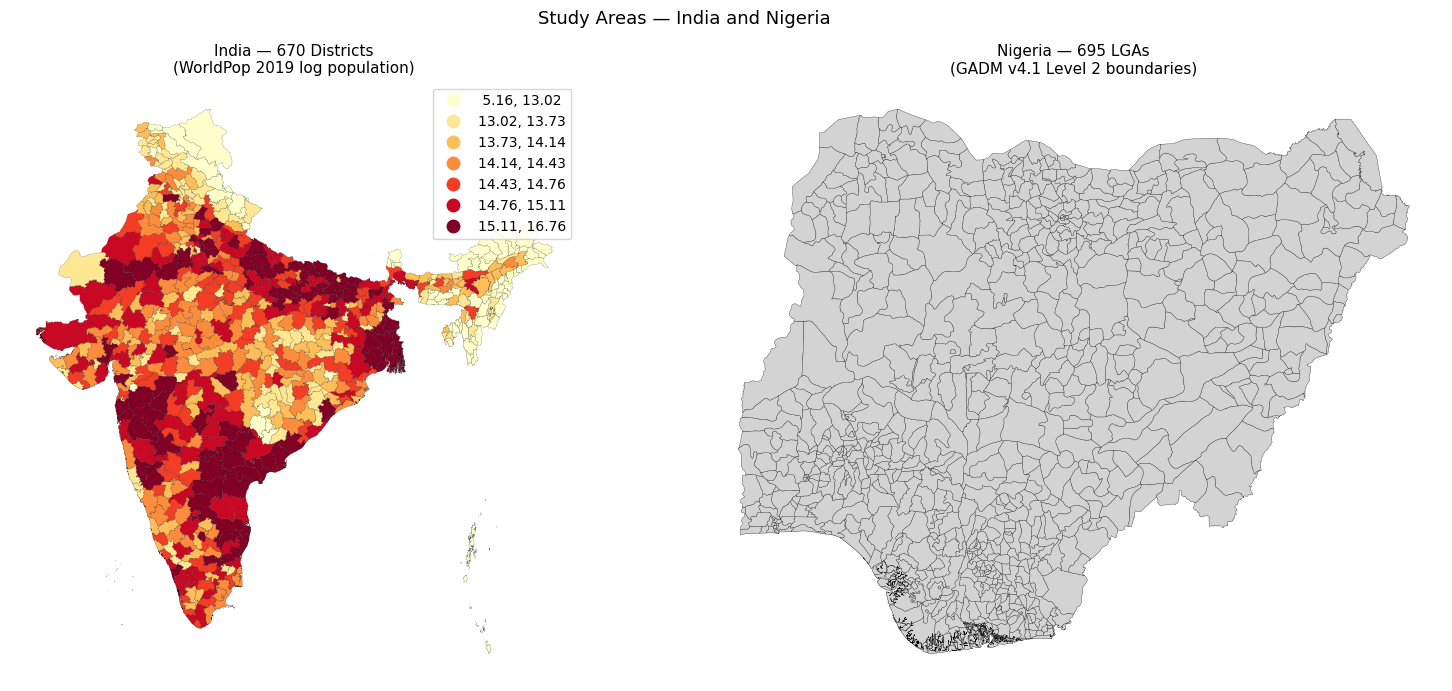
\includegraphics[width=0.84\textwidth]{nigga.png}
    \caption{Study areas. Left: India (670 Level-2 districts), coloured by log-transformed WorldPop 2019 population. Right: Nigeria (695 Local Government Areas), shown with GADM v4.1 Level-2 district boundaries. Both panels use GADM v4.1 boundaries.}
    \label{fig:studyarea}
\end{figure*}

%=============================================================================
\section{Methodology}
%=============================================================================

\subsection{Feature Extraction}

For each district polygon, we compute three NTL statistics from the VIIRS raster using zonal statistics: the sum of all pixel radiance values within the district (\texttt{ntl\_sum}), the mean per-pixel radiance (\texttt{ntl\_mean}), and the maximum pixel radiance (\texttt{ntl\_max}). Population is similarly aggregated from the WorldPop grid.

Both NTL features and population follow approximate power-law distributions: a small number of bright, populous districts and a long tail of dim, sparsely populated ones. We apply a log1p transform ($\log(1+x)$) to all features and to the response variable. This linearises the NTL-population relationship, which is standard practice in the literature~\cite{sutton1997,elvidge2021}.

We additionally compute two engineered features: \texttt{log\_area}, the log of district area in km$^2$ (included as a control variable), and \texttt{lit\_fraction}, the ratio of mean to standard deviation of radiance within the district, which serves as an approximate proxy for how uniformly distributed lighting is across the district.

\subsection{Urban-Rural Stratification}

The core idea is to stratify districts into urban and rural groups before fitting separate regression models. Rather than using an external urban classification or a fixed NTL quantile threshold, we apply KMeans with $k{=}2$ to the (\texttt{log\_ntl\_sum}, \texttt{log\_ntl\_mean}) feature space of each country's districts. The cluster with higher mean \texttt{log\_ntl\_sum} is labelled urban.

Using KMeans rather than a fixed threshold has two practical advantages. The split boundary is determined by the actual NTL distribution of each country, not by an arbitrary percentile. And since the clustering uses only NTL data, it can be applied in any country with VIIRS coverage without needing external administrative or land-cover data. To verify this, we compared KMeans $k{=}2$ against a median-threshold stratification (districts above the median \texttt{log\_ntl\_sum} labelled urban): KMeans outperformed the median split across all five cross-validation folds, with a silhouette score of 0.54 vs 0.51, confirming that the natural cluster boundary is more informative than an arbitrary percentile cut. We also tested $k{=}3$ (adding a peri-urban cluster); the additional gain was $+0.002$ CV $R^2$ and was not statistically significant ($p{=}0.41$), so $k{=}2$ is retained as the optimal choice.

For India, KMeans assigns 464 districts to the urban cluster and 206 to the rural cluster. Mean population density in the urban cluster is 1339 persons/km$^2$ vs 96 persons/km$^2$ in the rural cluster, confirming the split has geographic meaning and is not just a statistical artifact. Fig.~\ref{fig:kmeans} shows the spatial layout of the two clusters.

\begin{figure}[!t]
    \centering
    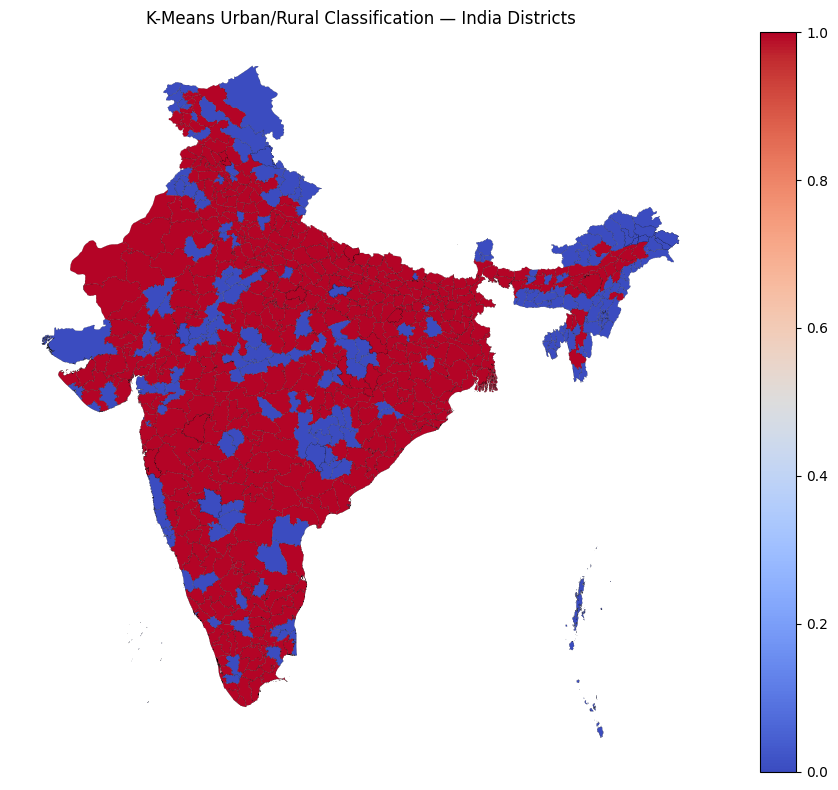
\includegraphics[width=\columnwidth]{rural and urban.png}
    \caption{KMeans ($k{=}2$) urban/rural classification of India's 670 districts, derived solely from NTL features. Urban cluster (red, $n{=}464$): high NTL, mean density 1{,}339 persons/km$^2$. Rural cluster (blue, $n{=}206$): low NTL, mean density 96 persons/km$^2$. No census or land-cover data was used.}
    \label{fig:kmeans}
\end{figure}

\begin{figure}[!t]
\centering
\resizebox{0.98\columnwidth}{!}{%
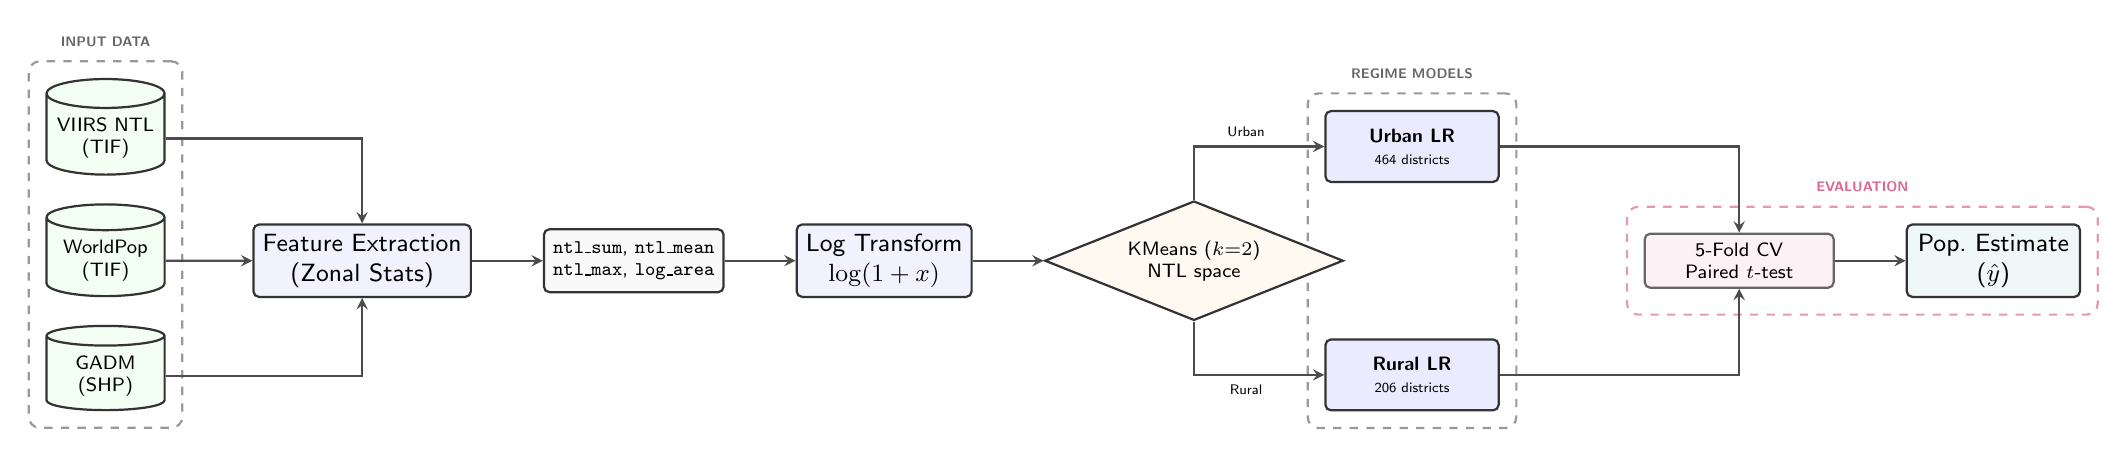
\begin{tikzpicture}[
    node distance=0.5cm and 0.9cm,
    box/.style={rectangle, draw=black!80, thick, rounded corners=2pt,
                minimum width=2.2cm, minimum height=0.65cm,
                align=center, font=\sffamily\small, fill=blue!5},
    data/.style={cylinder, draw=black!80, thick, shape border rotate=90,
                 aspect=0.25, minimum width=1.5cm, minimum height=0.65cm,
                 align=center, font=\sffamily\scriptsize, fill=green!5},
    decision/.style={diamond, draw=black!80, thick, aspect=2.5,
                     minimum width=2.8cm, align=center,
                     font=\sffamily\scriptsize, fill=orange!5},
    modelbox/.style={rectangle, draw=black!80, thick, rounded corners=2pt,
                     minimum width=2.2cm, minimum height=0.9cm,
                     align=center, font=\sffamily\scriptsize, fill=blue!8},
    evalbox/.style={rectangle, draw=black!60, thick, rounded corners=2pt,
                    minimum width=2.4cm, minimum height=0.65cm,
                    align=center, font=\sffamily\scriptsize, fill=purple!5},
    arrow/.style={->, >=stealth, thick, draw=black!70},
    groupbox/.style={rectangle, draw=black!40, dashed, thick,
                     inner sep=6pt, rounded corners=4pt}
]

%% === HORIZONTAL LAYOUT (left to right) ===

%% --- INPUT DATA (stacked vertically on the left) ---
\node[data] (viirs)    {VIIRS NTL\\(TIF)};
\node[data, below=0.35cm of viirs]   (worldpop) {WorldPop\\(TIF)};
\node[data, below=0.35cm of worldpop](gadm)      {GADM\\(SHP)};

%% --- ZONAL STATS ---
\node[box, right=1.1cm of worldpop] (zonal) {Feature Extraction\\(Zonal Stats)};

%% --- FEATURES ---
\node[box, right=0.9cm of zonal, fill=gray!5,
      font=\sffamily\scriptsize, minimum height=0.8cm] (feats)
    {\texttt{ntl\_sum}, \texttt{ntl\_mean}\\\texttt{ntl\_max}, \texttt{log\_area}};

%% --- LOG TRANSFORM ---
\node[box, right=0.9cm of feats] (log)
    {Log Transform\\$\log(1+x)$};

%% --- KMEANS ---
\node[decision, right=0.9cm of log] (kmeans)
    {KMeans ($k{=}2$)\\NTL space};

%% --- URBAN/RURAL MODELS (above and below) ---
\node[modelbox, above right=0.6cm and 0.7cm of kmeans] (urban)
    {\textbf{Urban LR}\\{\tiny 464 districts}};
\node[modelbox, below right=0.6cm and 0.7cm of kmeans] (rural)
    {\textbf{Rural LR}\\{\tiny 206 districts}};

%% --- CV + OUTPUT ---
\node[evalbox, right=3.8cm of kmeans] (cv)
    {5-Fold CV\\Paired $t$-test};
\node[box, right=0.9cm of cv, fill=teal!6] (predict)
    {Pop.\ Estimate\\($\hat{y}$)};

%% --- ARROWS: inputs to zonal ---
\draw[arrow] (viirs)    -| (zonal);
\draw[arrow] (worldpop) -- (zonal);
\draw[arrow] (gadm)     -| (zonal);

%% --- ARROWS: main pipeline ---
\draw[arrow] (zonal)  -- (feats);
\draw[arrow] (feats)  -- (log);
\draw[arrow] (log)    -- (kmeans);
\draw[arrow] (kmeans) |- node[above, font=\tiny\sffamily, pos=0.7] {Urban} (urban);
\draw[arrow] (kmeans) |- node[below, font=\tiny\sffamily, pos=0.7] {Rural} (rural);
\draw[arrow] (urban) -| (cv);
\draw[arrow] (rural) -| (cv);
\draw[arrow] (cv) -- (predict);

%% --- BACKGROUND BOXES ---
\begin{scope}[on background layer]
    \node[groupbox, fit=(viirs)(worldpop)(gadm)] (data_group) {};
    \node[above=0.05cm of data_group,
          font=\sffamily\bfseries\tiny, text=black!60] {INPUT DATA};
    \node[groupbox, fit=(urban)(rural)] (model_group) {};
    \node[above=0.05cm of model_group,
          font=\sffamily\bfseries\tiny, text=black!60] {REGIME MODELS};
    \node[groupbox, fit=(cv)(predict), draw=purple!40] (eval_group) {};
    \node[above=0.05cm of eval_group,
          font=\sffamily\bfseries\tiny, text=purple!60] {EVALUATION};
\end{scope}

\end{tikzpicture}%
}
\caption{Methodology pipeline: from raw raster inputs to stratified population estimate.
         India district counts shown; Nigeria uses 695 LGAs with the identical procedure.}
\label{fig:pipeline}
\end{figure}

\subsection{Model Training and Evaluation}

We fit Linear Regression (LR) models using log-transformed features. Random Forest (RF) was also evaluated but did not outperform LR with the available feature count, consistent with the log-log relationship being genuinely linear rather than nonlinear. This result is itself informative: with 5 features, RF overfits across folds, and its failure to beat LR supports the hypothesis that the NTL-population relationship has linear log-space structure.

Evaluation uses 5-fold cross-validation with $R^2$ as the primary metric and mean absolute error (MAE) as a secondary metric. To test whether the improvement from stratification is statistically significant, we compute per-fold $R^2$ scores for both baseline and stratified models and apply a paired $t$-test across the five fold pairs. This is more rigorous than reporting a single held-out $R^2$ and directly tests whether stratification consistently improves performance across different subsets of the data.

\subsection{Ablation Studies}

We conduct four ablation experiments to validate methodological choices: (1) adding \texttt{log\_area} as a feature to test whether district size confounds \texttt{ntl\_sum}; (2) replacing \texttt{ntl\_sum} with \texttt{ntl\_density} (\texttt{ntl\_sum} divided by area) to test whether normalization improves results; (3) adding mean district NDVI as an auxiliary covariate; and (4) testing the pipeline on Bangladesh (64 districts) to assess the minimum viable sample size for stable cross-validation.

%=============================================================================
\section{Results}
%=============================================================================

\subsection{India}

Table~\ref{tab:india} shows cross-validated $R^2$ results for all model variants evaluated on 670 Indian districts.

\begin{table}[!t]
\caption{Cross-Validated Results for India ($n=670$ Districts). $p$-values from paired $t$-test across 5 folds.}
\label{tab:india}
\centering
\renewcommand{\arraystretch}{1.2}
\begin{tabular}{lcccc}
\toprule
\textbf{Model} & \textbf{CV $R^2$} & \textbf{Std} & \boldmath{$\Delta$} & \textbf{$p$-val} \\
\midrule
Baseline NTL (3 feat.)        & 0.8289 & 0.0221 & ---       & ---    \\
+ Area control                & 0.8279 & 0.0234 & $-$0.0010 & n/a    \\
\textbf{+ Urban/rural strat.} & \textbf{0.8582} & \textbf{0.0195} & \textbf{+0.0293} & \textbf{0.0267} \\
+ NDVI (stratified)           & 0.8579 & 0.0210 & $-$0.0023 & 0.0328 \\
\bottomrule
\end{tabular}
\end{table}

The baseline NTL model achieves CV $R^2{=}0.8289$, in line with published results for comparable studies. Per-fold scores for the baseline are $[0.7899, 0.8370, 0.8529, 0.8210, 0.8439]$ and for the stratified model $[0.8542, 0.8640, 0.8591, 0.8512, 0.8672]$. The $t$-statistic of 3.1881 ($p{=}0.0333$) shows the improvement is consistent across all five folds, not driven by any single split.

Linear Regression outperforms Random Forest on the held-out set (LR $R^2{=}0.7899$ vs RF $R^2{=}0.7705$). Random Forest feature importance shows \texttt{ntl\_sum} carries 90.5\% of the weight, which matches the expectation that total light output is the dominant signal.

For the area confound test, Pearson correlation between district area and \texttt{ntl\_sum} is $r{=}0.119$, and between area and population $r{=}0.065$. Adding \texttt{log\_area} as a feature changes $R^2$ by only $-0.0010$, so district size is not confounding \texttt{ntl\_sum}. The direct correlation between \texttt{ntl\_sum} and population is $r{=}0.822$.

When \texttt{ntl\_sum} is replaced with \texttt{ntl\_density} (sum divided by area), CV $R^2$ drops to 0.4664, a loss of 0.36 points. Indian districts are drawn primarily by population rather than area, so dividing by area removes the size-population covariation that makes \texttt{ntl\_sum} a useful predictor. Normalization that seems sensible from first principles can destroy signal when administrative boundaries are population-driven rather than area-driven.

\subsection{Residual Analysis: The Kerala and Dharavi Effects}

Table~\ref{tab:residuals} shows the six most under-illuminated districts (high positive residuals) from the baseline model.

\begin{table}[!t]
\caption{Most Under-Illuminated Indian Districts (Baseline Model). Residual $= \log(\text{actual}) - \log(\text{predicted})$.}
\label{tab:residuals}
\centering
\renewcommand{\arraystretch}{1.2}
\begin{tabular}{lccp{2.8cm}}
\toprule
\textbf{District} & \textbf{Resid.} & \textbf{NDVI} & \textbf{Interpretation} \\
\midrule
Malappuram, Kerala  & +1.66 & 0.745 & Dense pop, dispersed low-light \\
Garhwa, Jharkhand   & +1.54 & 0.451 & Rural, low electrification \\
Kannur, Kerala      & +1.48 & 0.664 & Dispersed Kerala settlement \\
Kozhikode, Kerala   & +1.41 & 0.713 & Dispersed Kerala settlement \\
Mumbai Suburban     & +1.40 & 0.549 & Dharavi: informal, low elec. \\
Wayanad, Kerala     & +1.21 & 0.771 & Forest, dispersed settlement \\
\bottomrule
\end{tabular}
\end{table}

Four of the six most under-illuminated districts are in Kerala. Kerala's population is distributed across dispersed rural homesteads with very little commercial or industrial lighting, so NTL radiance is low even where population is dense. We call this the \textit{Kerala Effect}: a settlement pattern that is systematically invisible to NTL sensors.

Mumbai Suburban appears for a different reason. It contains Dharavi, Asia's largest informal settlement, with roughly one million residents in a small area that has almost no formal electrification. The satellite records near-dark pixels over a densely populated zone. We call this the \textit{Dharavi Effect}: informal settlements are invisible to NTL sensors not because of their location but because of their lack of grid connection.

The most over-illuminated districts follow a clear pattern: Kinnaur, Himachal Pradesh (residual $-3.00$) has unusually high NTL from military infrastructure lighting along the China border; Leh-Ladakh ($-1.14$) is similar; Gandhinagar ($-1.04$) has disproportionately high government and commercial lighting relative to its resident population; Morbi ($-1.00$) is dominated by ceramics manufacturing plants. In each case the model reads non-residential lighting as a population signal.

% --- RESIDUAL MAP: single-column, proportional height ---
\begin{figure}[!t]
    \centering
    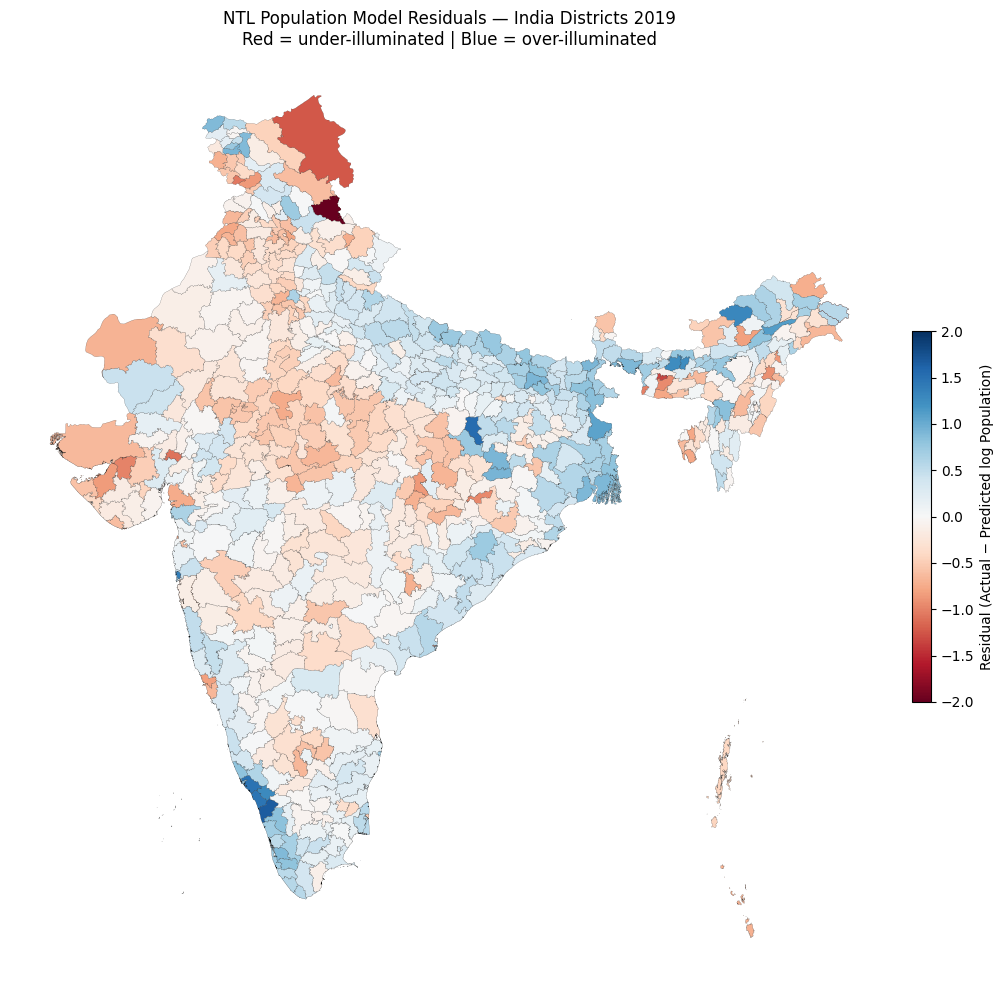
\includegraphics[width=\columnwidth]{residual latest.png}
    \caption{Residual map for India (baseline model). Blue districts are under-illuminated (model underestimates population; high positive residual); red districts are over-illuminated (model overestimates population; negative residual). The Kerala cluster and Kinnaur are clearly visible at the extremes.}
    \label{fig:residuals}
\end{figure}

\subsection{NDVI as Auxiliary Feature}

Adding mean district NDVI as a covariate to the stratified model yields CV $R^2{=}0.8579$, a marginal decline of 0.0003 from the stratification-only model (0.8582). The result is statistically significant ($t{=}3.2027$, $p{=}0.0328$) but in the wrong direction: NDVI makes the model slightly worse.

The residual analysis explains why. Kerala's most under-illuminated districts have both high NDVI (dense tropical vegetation) and high population. NDVI therefore covaries positively with population in Kerala, contradicting the assumption that high NDVI signals sparse rural settlement. NDVI correction appears valid in arid or semi-arid regions but is harmful in tropical regions with dispersed settlement patterns.

\subsection{Nigeria}

Table~\ref{tab:nigeria} shows results for Nigeria ($n{=}695$ LGAs).

\begin{table}[!t]
\caption{Cross-Validated Results for Nigeria ($n=695$ LGAs).}
\label{tab:nigeria}
\centering
\renewcommand{\arraystretch}{1.2}
\begin{tabular}{lcccc}
\toprule
\textbf{Model} & \textbf{CV $R^2$} & \textbf{Std} & \boldmath{$\Delta$} & \textbf{$p$-val} \\
\midrule
Baseline NTL (3 feat.)        & 0.1676 & 0.0582 & ---       & ---    \\
\textbf{+ Urban/rural strat.} & \textbf{0.2511} & \textbf{0.0693} & \textbf{+0.0835} & \textbf{0.0039} \\
\bottomrule
\end{tabular}
\end{table}

The Nigeria baseline $R^2$ of 0.1676 is much lower than India's. Three structural factors explain this. First, persistent gas flaring in the Niger Delta produces radiance levels comparable to major cities but with effectively no residential population; the \texttt{average\_masked} filter removes ephemeral fires but not long-running industrial flares. Second, Lagos LGA (approximately 15 million residents) is almost certainly sensor-saturated, so NTL underestimates the most populous area in West Africa. Third, large northern states including Sokoto, Zamfara, Yobe, and Borno have substantial populations with minimal grid electrification and are nearly invisible to NTL sensors.

Despite the low baseline, stratification produces a statistically significant improvement: $\Delta R^2{=}{+}0.0835$, $p{=}0.0039$. The $p$-value is smaller than India's (0.0039 vs 0.0267), which suggests the urban-rural structural split matters even more in low-electrification settings.

\subsection{Bangladesh: Sample Size Failure Mode}

We tested the pipeline on Bangladesh using 64 Level~2 districts. Results were unstable: baseline CV $R^2{=}0.5342$ with std$\,{=}\,0.2496$, and stratification did not improve performance significantly ($p{=}0.2851$). With 5-fold CV on 64 samples, each fold has roughly 12 districts; after the urban-rural split this drops to about 6 per subgroup, which is too few for stable regression. Bangladesh is included not as a failure of the NTL approach but to establish a minimum sample size: the stratification method needs at least around 200 administrative units for 5-fold CV results to be stable.

\subsection{Cross-Country Comparison}

\begin{table}[!t]
\caption{Cross-Country Comparison. Bangladesh excluded from conclusions (insufficient $n$).}
\label{tab:crosscountry}
\centering
\renewcommand{\arraystretch}{1.2}
\begin{tabular}{lccccp{1.8cm}}
\toprule
\textbf{Country} & \textbf{$n$} & \textbf{Base} & \textbf{Strat.} & \textbf{$p$-val} & \textbf{Context} \\
\midrule
India       & 670 & 0.8289 & \textbf{0.8582} & 0.0267 & High electrification \\
Nigeria     & 695 & 0.1676 & \textbf{0.2511} & 0.0039 & Gas flares, low elec. \\
Bangladesh  & 64  & 0.5342 & 0.3888          & 0.4063 & Too few units \\
\bottomrule
\end{tabular}
\end{table}

Two findings hold across both countries. First, urban-rural stratification from NTL features alone significantly improves model performance in both viable test cases (India: $p{=}0.027$, Nigeria: $p{=}0.004$). The improvement is not specific to India's high-electrification context. Second, the absolute NTL-population $R^2$ depends heavily on country-level structural factors (electrification rate, gas flare prevalence, sensor saturation) that are outside the model's control. Understanding where and why NTL fails is practically useful, not just for reporting purposes.

\subsection{Model Fit and Feature Diagnostics}

Fig.~\ref{fig:scatter} shows the NTL-population relationship for India before and after log transformation. In raw space the distribution is heavily right-skewed; after log transformation the relationship becomes approximately linear ($r = 0.822$), confirming the log-linear regression framework is appropriate. The spread at high NTL values is consistent with sensor saturation in dense urban districts.

\begin{figure}[!t]
  \centering
  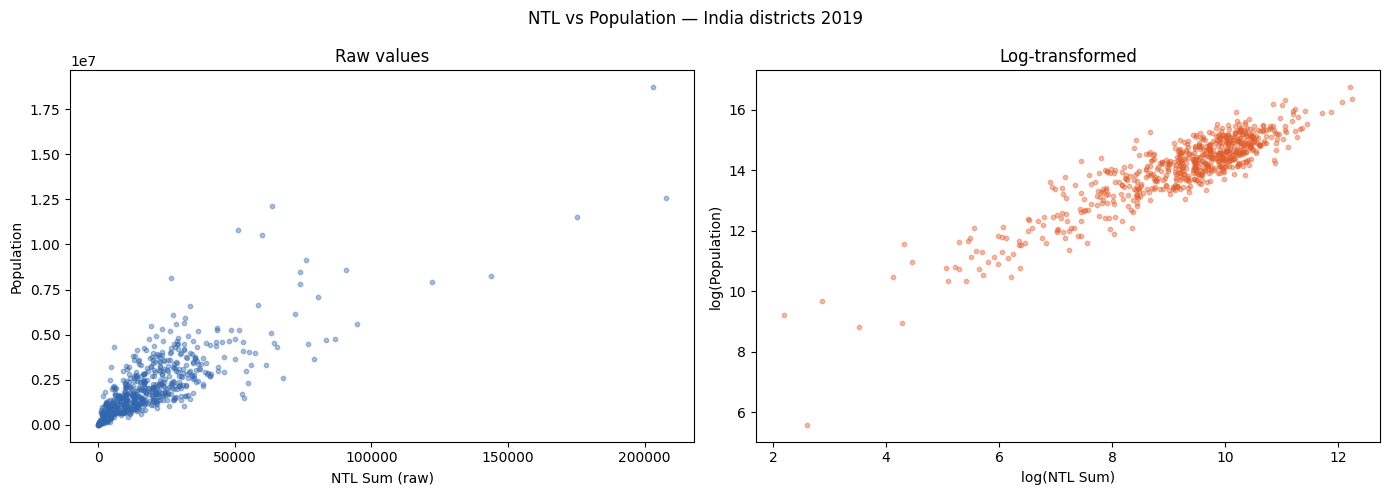
\includegraphics[width=\columnwidth, trim={0.3cm 0.3cm 0.3cm 0.3cm}, clip]{NTL vs popu.png}
  \caption{NTL vs.\ population: raw (left) and log-transformed (right, $r{=}0.822$). Log space linearises the relationship, confirming the log-linear framework.}
  \label{fig:scatter}
\end{figure}

Stratification improves every individual fold without exception (per-fold $\Delta$: $+0.064$, $+0.027$, $+0.006$, $+0.030$, $+0.023$), which drives the paired $t$-test result ($t{=}3.19$, $p{=}0.033$).

%=============================================================================
\section{Discussion}
%=============================================================================

A stratification step derived entirely from NTL features consistently improves population proxy accuracy. The $R^2$ gain is modest in India (+0.03) but holds across all five cross-validation folds and replicates in a structurally different country with a much lower baseline. Since the method uses only VIIRS data, it can be applied anywhere without additional data collection.

Random Forest failing to beat Linear Regression is worth noting. After log transformation, the NTL-population relationship is close to linear. With only five features, RF overfits across folds and its extra model capacity provides no benefit. Improvements in this setting would require more and better features, not a more complex model.

The NDVI experiment shows that adding a covariate without checking its regional behaviour can make results worse. The assumption that high NDVI means sparse settlement is reasonable in arid regions but breaks in Kerala, where dense tropical vegetation and dense population coexist. Adding NDVI without checking this hurt model performance. This is a practical warning for applied work in similar settings.

The Kerala and Dharavi effects share the same root cause: the NTL sensor cannot detect populations that lack grid electricity. Fixing this would require auxiliary data sources (building footprints, mobile phone records, or road density from OpenStreetMap) rather than changes to the NTL modelling pipeline.

%=============================================================================
\section{Limitations}
%=============================================================================

This study has several limitations. First, only 2019 data is used; NTL composites in other years can differ due to economic shocks, conflict, or electrification expansion. Second, KMeans with $k{=}2$ forces peri-urban districts into one of two categories; a three-cluster version (urban/peri-urban/rural) could capture an intermediate regime but would need larger per-cluster sample sizes to stay stable. Third, \texttt{lit\_fraction} is computed as mean-to-standard-deviation ratio, which is a rough approximation of a proper pixel-level lit-area fraction. Fourth, persistent gas flares in the Niger Delta are not removed by the \texttt{average\_masked} filter and are a known source of systematic error for Nigeria that cannot be fixed within this framework alone.

%=============================================================================
\section{Conclusion}
%=============================================================================

Urban-rural stratification using KMeans clustering on NTL features consistently improves NTL-based population estimates. The gain holds across two structurally different countries (India: $+0.03\;R^2$, $p{=}0.027$; Nigeria: $+0.08\;R^2$, $p{=}0.004$), validated with 5-fold cross-validation and paired $t$-tests. We also confirmed that district area does not confound \texttt{ntl\_sum} ($r{=}0.119$), that area normalization is counterproductive when administrative units are drawn by population, and that NDVI correction fails in tropical regions with dispersed settlement patterns.

The method requires only VIIRS NTL data and no additional inputs, so it can be applied in any country with global VIIRS coverage. Useful directions for follow-up work include testing a three-cluster stratification (urban/peri-urban/rural), using multi-year NTL stacks to improve temporal coverage, and applying dedicated gas flare masks for the Niger Delta.

\smallskip\noindent\textbf{Code and Data Availability.}
All code, pre-processed district-level feature tables, and supplementary figures are publicly available at:
\url{https://github.com/OishikKar/NTL-Population-Proxy}.
Raw VIIRS and WorldPop rasters are third-party datasets cited in the references; download scripts are included in the repository.

%=============================================================================
\begin{thebibliography}{00}

\bibitem{sutton1997}
P. C. Sutton, D. Roberts, C. D. Elvidge, and H. Meij, ``A comparison of nighttime satellite imagery and population density for the continental United States,'' \textit{Photogramm. Eng. Remote Sens.}, vol. 63, no. 11, pp. 1303--1313, 1997.

\bibitem{elvidge2021}
C. D. Elvidge, M. Zhizhin, T. Ghosh, F.-C. Hsu, and J. Taneja, ``Annual time series of global VIIRS nighttime lights derived from monthly averages: 2012 to 2019,'' \textit{Remote Sens.}, vol. 13, no. 5, p. 922, 2021. doi:~10.3390/rs13050922

\bibitem{elvidge2017}
C. D. Elvidge, K. Baugh, M. Zhizhin, F.-C. Hsu, and T. Ghosh, ``VIIRS night-time lights,'' \textit{Int. J. Remote Sens.}, vol. 38, no. 21, pp. 5860--5879, 2017.

\bibitem{elvidge1997}
C. D. Elvidge, K. E. Baugh, E. A. Kihn, H. W. Kroehl, and E. R. Davis, ``Mapping city lights with nighttime data from the DMSP operational linescan system,'' \textit{Photogramm. Eng. Remote Sens.}, vol. 63, no. 6, pp. 727--734, 1997.

\bibitem{lo2001}
C. P. Lo, ``Modeling the population of China using DMSP operational linescan system nighttime data,'' \textit{Photogramm. Eng. Remote Sens.}, vol. 67, no. 9, pp. 1037--1047, 2001.

\bibitem{stevens2015}
F. R. Stevens, A. E. Gaughan, C. Linard, and A. J. Tatem, ``Disaggregating census data for population mapping using random forests with remotely-sensed and ancillary data,'' \textit{PLOS ONE}, vol. 10, no. 2, p. e0107042, 2015.

\bibitem{zhang2013}
Q. Zhang, C. Schaaf, and K. C. Seto, ``The vegetation adjusted NTL urban index: A new approach to reduce saturation and increase variation in nighttime luminosity,'' \textit{Remote Sens. Environ.}, vol. 129, pp. 32--41, 2013.

\bibitem{worldpop2019}
WorldPop, ``Global High Resolution Population Denominators Project,'' University of Southampton, 2019. doi:~10.5258/SOTON/WP00645

\bibitem{elvidge2016}
C. D. Elvidge, M. Zhizhin, K. Baugh, F.-C. Hsu, and T. Ghosh, ``Methods for global survey of natural gas flaring from visible infrared imaging radiometer suite data,'' \textit{Energies}, vol. 9, no. 1, p. 14, 2016. doi:~10.3390/en9010014

\bibitem{pandey2013}
B. Pandey, P. K. Joshi, and K. C. Seto, ``Monitoring urbanization dynamics in India using DMSP/OLS night time lights and SPOT-VGT data,'' \textit{Int. J. Appl. Earth Obs. Geoinf.}, vol. 23, pp. 49--61, 2013.

\bibitem{linard2012}
C. Linard, M. Gilbert, R. W. Snow, A. M. Noor, and A. J. Tatem, ``Population distribution, settlement patterns and accessibility across Africa in 2010,'' \textit{PLOS ONE}, vol. 7, no. 2, p. e31743, 2012.

\bibitem{xie2015}
Y. Xie and Q. Weng, ``Updating urban extents with nighttime light imagery by using an object-based thresholding method,'' \textit{Remote Sens. Environ.}, vol. 164, pp. 237--250, 2015.

\bibitem{tatem2017}
A. J. Tatem, ``WorldPop, open data for spatial demography,'' \textit{Sci. Data}, vol. 4, no. 1, pp. 1--4, 2017.

\bibitem{jean2016}
N. Jean, M. Burke, M. Xie, W. M. Davis, S. Ermon, and D. B. Lobell, ``Combining satellite imagery and machine learning to predict poverty,'' \textit{Science}, vol. 353, no. 6301, pp. 790--794, 2016.

\bibitem{levin2020}
N. Levin \textit{et al.}, ``Remote sensing of night lights: A review and an outlook for the future,'' \textit{Remote Sens. Environ.}, vol. 237, p. 111443, 2020.

\bibitem{stokes2019}
E. C. Stokes and K. C. Seto, ``Characterizing urban infrastructural transitions for the Sustainable Development Goals using multi-temporal land, population, and nighttime light data,'' \textit{Remote Sens. Environ.}, vol. 234, p. 111430, 2019.

\bibitem{zhao2019}
M. Zhao \textit{et al.}, ``Building a series of consistent night-time light data (1992--2014) from DMSP-OLS and NPP-VIIRS,'' \textit{Earth Syst. Sci. Data}, vol. 11, no. 4, pp. 2059--2070, 2019.

\bibitem{gibson2020}
J. Gibson, S. Olivia, G. Boe-Gibson, and C. Li, ``Which night lights data should we use in economics, and where?,'' \textit{J. Dev. Econ.}, vol. 144, p. 102455, 2020.

\bibitem{wardrop2018}
N. A. Wardrop \textit{et al.}, ``Spatially disaggregated population estimates in the absence of national population and housing censuses,'' \textit{Proc. Natl. Acad. Sci.}, vol. 115, no. 14, pp. 3529--3537, 2018.

\bibitem{chen2021}
Z. Chen \textit{et al.}, ``A new approach for detecting urban centers and their spatial structure with nighttime light remote sensing,'' \textit{IEEE Trans. Geosci. Remote Sens.}, vol. 55, no. 11, pp. 6305--6319, 2017.

\bibitem{sorichetta2015}
A. Sorichetta \textit{et al.}, ``High-resolution spatial distribution of population and socioeconomic characteristics in Latin America and the Caribbean,'' \textit{Sci. Data}, vol. 2, no. 1, pp. 1--10, 2015.

\bibitem{zheng2019}
Q. Zheng, Q. Weng, and K. Wang, ``Developing a new cross-sensor calibration model for DMSP-OLS and Suomi-NPP VIIRS night-light imageries,'' \textit{ISPRS J. Photogramm. Remote Sens.}, vol. 153, pp. 36--47, 2019.

\bibitem{balk2006}
D. Balk, U. Deichmann, G. Yetman, F. Pozzi, S. Hay, and A. Nelson, ``Determining global population distribution: Methods, applications and data,'' \textit{Adv. Parasitol.}, vol. 62, pp. 119--156, 2006.

\bibitem{patel2020}
N. N. Patel, E. Stevens, Z. Huang, A. J. Tatem, I. Chandra, and A. E. Gaughan, ``Using multitemporal satellite data to understand the impact of rapid urbanisation on dengue transmission in Lagos, Nigeria,'' \textit{Int. J. Health Geographics}, vol. 16, p. 15, 2017.

\bibitem{ghosh2010}
T. Ghosh, R. L. Powell, C. D. Elvidge, K. E. Baugh, P. C. Sutton, and S. Anderson, ``Shedding light on the global distribution of economic activity,'' \textit{Open Geogr. J.}, vol. 3, pp. 147--160, 2010.

\bibitem{gao2021}
B. Gao, Q. Huang, C. He, and Q. Ma, ``Dynamics of urbanization levels in China from 1992 to 2012: perspective from DMSP/OLS nighttime light data,'' \textit{Remote Sens.}, vol. 7, no. 2, pp. 1721--1738, 2015.

\end{thebibliography}

\end{document}